\begin{center}
\large\noindent\fbox{
	\parbox{\textwidth}{
	 Ripetere una procedura analoga a quella del precedente esercizio utilizzando il metodo di Gauss-Seidel.
}
}\end{center}

\noindent Il codice Matlab utilizzato per realizzare il grafico \'e il seguente:

\lstinputlisting[language=Matlab]{Codici/Cap6/Soluzione4_Cap6.m}

\vspace*{0.5cm}

\lstinputlisting[language=Matlab]{Codici/Cap6/gaussSeidel.m}

\vspace*{0.5cm}

\lstinputlisting[language=Matlab]{Codici/Cap6/trisolveInfGaussSeidel.m}

\noindent Grafico risultante: 

\begin{figure}[H]
	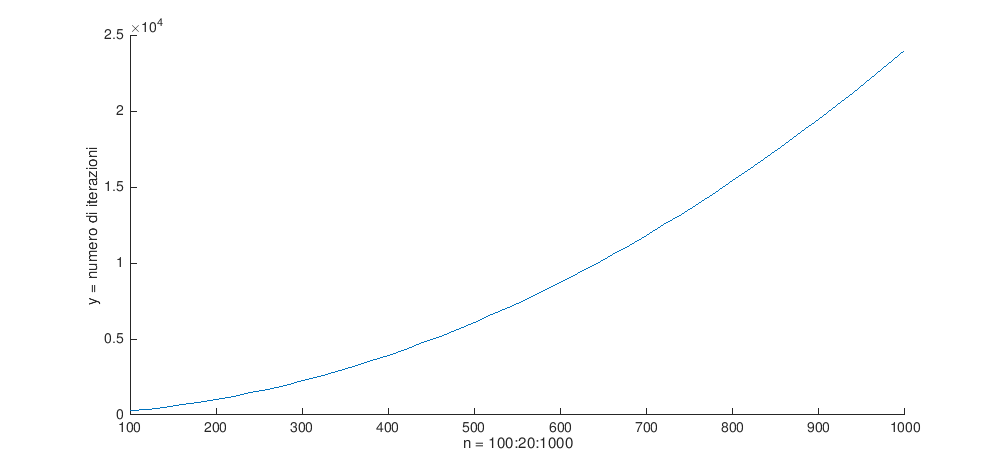
\includegraphics[width=\textwidth]{Codici/Cap6/es4cap6}
\end{figure}
